% template created by: Russell Haering. arr. Joseph Crop
\documentclass[12pt,letterpaper]{article}
\usepackage{anysize}
\usepackage{cite}
\usepackage{amsmath,amssymb,amsfonts}
\usepackage{algorithm}
\usepackage[noend]{algpseudocode}
\usepackage{graphicx}
\usepackage{multirow}
\usepackage{listings}
\usepackage{xcolor}


\marginsize{2cm}{2cm}{1cm}{1cm}

\lstset{ framexleftmargin=9mm, frame=shadowbox,tabsize = 4}

\begin{document}

\begin{titlepage}
    \vspace*{4cm}
    \begin{flushright}
    {\huge
        ECE 375 Lab 6\\[1cm]
    }
    {\large
    	Timer/Counters
    }
    \end{flushright}
    \begin{flushleft}
    Lab session: 015
    
    Time: 12:00-13:50
    \end{flushleft}
    \begin{flushright}
    Author: Astrid Delestine

    Programming partner: Lucas Plastid 

    \vfill
    \rule{5in}{.5mm}\\
    TA Signature
    \end{flushright}

\end{titlepage}

\section{Introduction}
%This is the first Lab in the ECE 375 series and it covers the setup and compilation of an AVR Assembly Program. The student will learn how how to use the sample Basic Bump Bot assembly file and send the binaries to the AVR Microcontroller board. For the second part of the lab the student will be expected to download and compile the included C sample program and from it learn how to configure the I/O ports of the ATmega32U4 Microcontroller. The student will then write their own C program and upload it to the Microcontroller to verify that it runs as expected. The provided programs have been attached in the source code section of this report.


\section{Design}

\begin{figure}[h]
	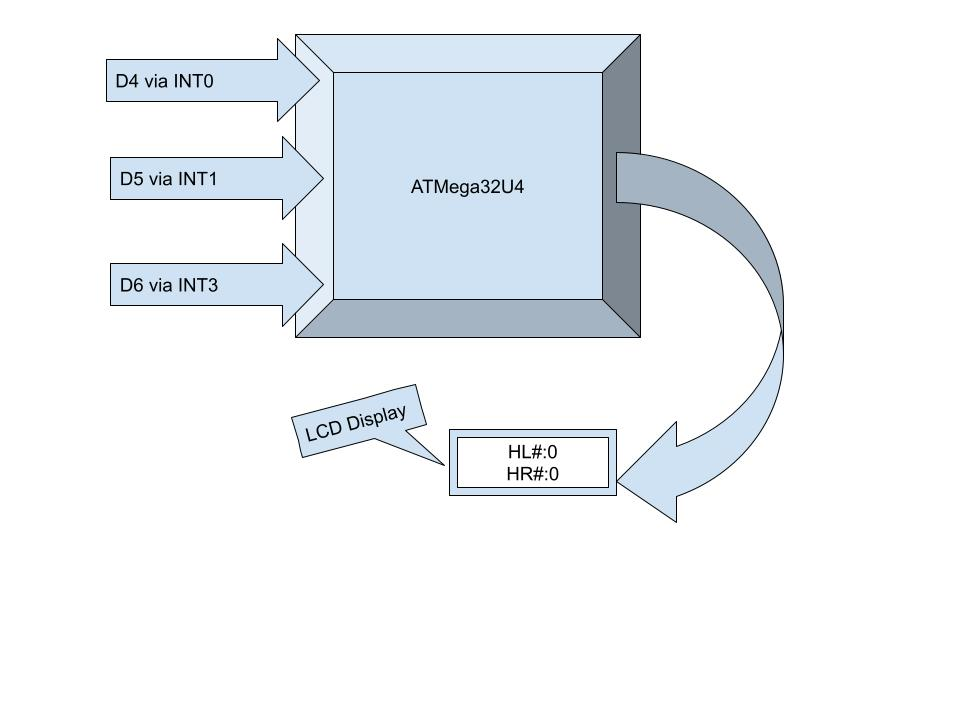
\includegraphics[width=12cm, height=10cm]{Block Diagram L5.jpg}
	\centering
\end{figure}
	
\section{Assembly Overview}
As for the Assembly program an overview can be seen below. 

\subsection{Internal Register Definitions and Constants}


\subsection{Interrupt Vectors}




\subsection{Initialization Routine}


\subsection{Main Routine}



\subsection{Subroutines}
	\subsection{INCSPD}
	
	
	\subsection{DECSPD}
	

	\subsubsection{MAXSPD}

	 
	
	\subsubsection{WRITESPD}

	
	\subsubsection{Wait}
	The standard wait function.
	
	

\section{Testing}
Tested Each button press and compared to external calculations.
\begin{table}[h]
	\centering
	\begin{tabular}{|l|l|l|ll}
		\cline{1-3}
		Case & Expected & Actual meet expected &  &  \\ \cline{1-3}
	d4	&an increment on the LCD, and the bump bot right hit function to be called&	\checkmark  &  \\ \cline{1-3}
	d5	&an increment on the LCD, and the bump bot left hit function to be called&	\checkmark	&  \\ \cline{1-3}
	d6	&The two numbers listed on the screen reset&	\checkmark  &  \\ \cline{1-3}
	d7	&nothing&	\checkmark	&  \\ \cline{1-3}
	
%		&          &                      &  &  \\ \cline{1-3}
	\end{tabular}
\caption{Assembly Testing Cases}
\end{table}

\section{Study Questions}
\begin{enumerate}
    \item
    In this lab, you used the Fast PWM mode of 16-bit Timer/Counter, which is only one of many possible ways to implement variable speed on a Tek-Bot. Suppose instead that you used Normal mode, and had it generate an interrupt for every overflow. In the overflow ISR, you manually toggled both Motor Enable pins of the TekBot, and wrote a new value into the Timer/Counter’s register. (If you used the correct sequence of values, you would be manually performing PWM.) Give a detailed assessment (in 1-2 paragraphs) of the advantages and disadvantages of this new approach, in comparison to the PWM approach used in this lab.
    
    
    \item 
    the previous question outlined a way of using a single 16-bit Timer/Counter in Normal mode to implement variable speed. How would you accomplish the same task (variable TekBot speed) using in CTC mode? Provide a rough-draft sketch of the Timer/Counter-related parts of your design, using either a flow chart or some pseudocode (but not actual assembly code)
    
    \begin{figure}[h]
    	 A drawing of how this might work can be seen below
    	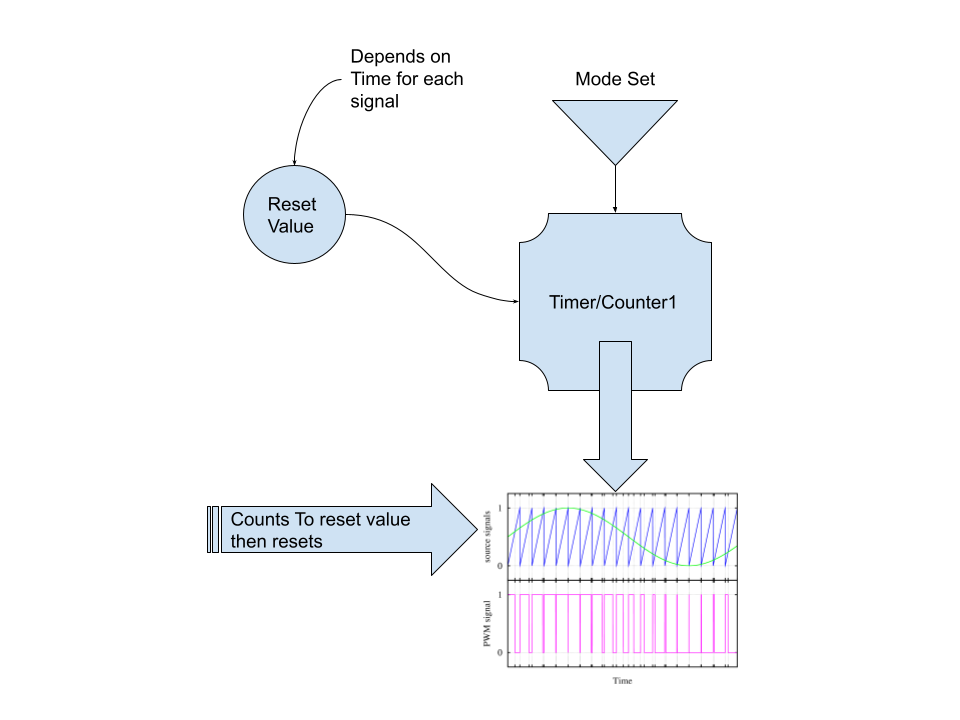
\includegraphics[width=12cm, height=10cm]{q2Drawing.png}
    	\centering
    \end{figure}
   
    

    
    \item 
	In the next lab, you will be utilizing Timer/Counter1, which can make use of several 16 bit timer registers. The datasheet describes a particular manner in which these registers must be manipulated. To illustrate the process,
	write a snippet of assembly code that configures OCR1A with a value of 0x1234. For the sake of simplicity, you may assume that no interrupts are triggered during your code’s operation.
	
	ldi mpr, High(0x1234) ; You have to set the high first because if you set the low first, you will not actually have set the lower bits correctly.
	sts OCR1AH, mpr
	ldi mpr Low(0x1234)
	sts OCR1AL, mpr
	
    
    \item
    Each ATmega32U4 USART module has two flags used to indicate its current transmitter state: the Data Register Empty (UDRE) flag and Transmit Complete (TXC) flag. What is the difference between these two flags, and which one always gets set first as the transmitter runs? You will probably need to read about the Data Transmission process in the datasheet (including looking at any relevant USART diagrams) to answer this question.
    
    The UDRE flag determines if the USART bus is ready to reccive data. It is set to a 1 when the register of the USART is empty. On the other hand the TXC flag is set when the entire message has been sent. Thus we know that the UDRE flag is set first as the transmitter runs, waiting for the transmit buffer to be empty before loading it with new data.
    
    \item 
    Each ATmega32U4 USART module has one flag used to indicate its current receiver state (not including the error flags). For USART1 specifically, what is the name of this flag, and what is the interrupt vector address for the
    interrupt associated with this flag? This time, you will probably need to read about Data Reception in the datasheet to answer this question
    
    The name of the flag for USART1 is UDRE1, and its interrupt vector location is \$0034 
    
       
    
\end{enumerate}

\section{Difficulties}
This Lab challenged the thinking power of implementation of ideas we have learned in lecture. It was not too difficult however did require refrenceing both the AVR manual and the atmega32u4 datasheet.

\section{Conclusion}
In conclusion, this lab introduced and allowed the student to understand many more aspects of how to program a function using interrupts and modify an existing program to work with an LCD in conjunction with those interrupts. This lab proves that the student is learning how to modify certain code structures and is becoming more fluent in the AVR programming scheme

\pagebreak

\section{Source Code}%
\lstinputlisting
[
caption=Assembely Script,
language={[x86masm]Assembler},
numbers =left,
rulesepcolor=\color{blue}
]{../Lab6Assm/Lab6Assm/Astrid_Delestine_and_Lucas_Plaisted_Lab6_sourcecode.asm}





\end{document}